\chapter{Introducción}

La calidad de los sistemas de software típicamente se define alrededor de varios aspectos, tales como confiabilidad, usabilidad, eficiencia, etc. Entre ellos, la confiabilidad es generalmente considerada una característica fundamental en lo que respecta a la calidad del software, y de gran interés en el proceso de desarrollo de software [0]. 

Analizar la calidad del software está fuertemente relacionado con la tarea de encontrar defectos en el mismo, es decir, identificar algún comportamiento actual del software que difiera del comportamiento esperado. En este sentido, si se considera un determinado dato de entrada para un sistema, el desafío de distinguir el comportamiento correcto de uno incorrecto es conocido como el problema del oraculo []. Es esperable que esta tarea se pueda realizar con el menor costo posible y con los mayores beneficios, garantizando que el sistema funcione correctamente para distintos valores de entrada. 
Se han introducido técnicas para oráculos automáticos como modelado, especificaciones, desarrollo guiado por contratos, y testing metamorfico. Aún así existen casos donde ninguna de estas técnicas son adecuadas, por lo que la intervención manual del desarrollador es necesaria.

Las especificaciones de software pueden aparecer de diversas maneras. A nivel de código fuente, cuando están presentes, generalmente se manifiestan o bien como comentarios, es decir, descripciones informales en lenguaje natural de lo que se supone que debe hacer el software, o más formalmente como aserciones de programas, es decir, declaraciones (normalmente ejecutables) que capturan propiedades que el software debe satisfacer en ciertos puntos durante su ejecución. Las especificaciones como comentarios son más comunes, pero tiene la desventaja de que no pueden utilizarse de manera directa para el análisis automático de confiabilidad. 
Deido a esta situación, el problema de inferencia de especificaciones (un caso especial del conocido problema del oráculo [Barr et al. 2015]), es decir, el problema de generar una descripción formal del comportamiento del software a partir de elementos existentes (documentación, código fuente, etc.), ha recibido una atención cada vez mayor por parte de la comunidad de Ingeniería de Software.

En las últimas décadas, con el objetivo de ayudar a los desarrolladores a equipar las implementaciones con especificaciones, se han desarrollado una variedad de técnicas de inferencia automática de aserciones de regresión, es decir, aserciones que capturan el comportamiento actual del software. Estas técnicas, generalmente basadas en observaciones de ejecuciones del software bajo análisis, pueden producir distintos tipos de aserciones de regresión. Por ejemplo, algunas técnicas de generación automática de tests [Fraser & Arcuri 2011, Pacheco & Ernst 2007] incorporan mecanismos para producir aserciones de test, es decir, aserciones que capturan propiedades válidas en un escenario (test) específico. Por otro lado, otras técnicas de inferencia de especificaciones [Ernst et al. 2007, Le & Lo 2018, Molina et al. 2019, Molina et al. 2021, Molina et al. 2022, Terragni et al. 2020] son capaces de inferir aserciones de contratos, es decir, aserciones más generales asociadas con elementos de contratos como precondiciones, postcondiciones e invariantes [Meyer 1992].

\section{Problema}

La principal hipótesis de trabajo es que el tipo de aserciones de regresión utilizadas en testing de regresión, ya sean aserciones de test o aserciones de contratos, puede tener un impacto considerable en la efectividad del análisis para detectar defectos producidos por cambios en el software.

El objetivo principal de este trabajo es el estudio y análisis de la efectividad de distintas aserciones de regresión para detectar errores durante la tarea de testing de regresión. Esencialmente, se desea analizar la efectividad de las aserciones de test en comparación con las aserciones de contratos. Para esta tarea, se propone, para diversos casos de estudio de la literatura, simular escenarios de testing de regresión utilizando, por un lado, aserciones de test, y por otro, aserciones de contratos, generadas automáticamente. 

En particular se pone el foco en las aserciones generadas por herramientas del estado del arte de generación automática de tests como Randoop[0] y Daikon[0]. 

A modo de ejemplo consideremos la implementación de nodo de listas doblemente enlazadas con su método insertRight en el lenguaje de programación Java.

\begin{figure}[ht]
\centering
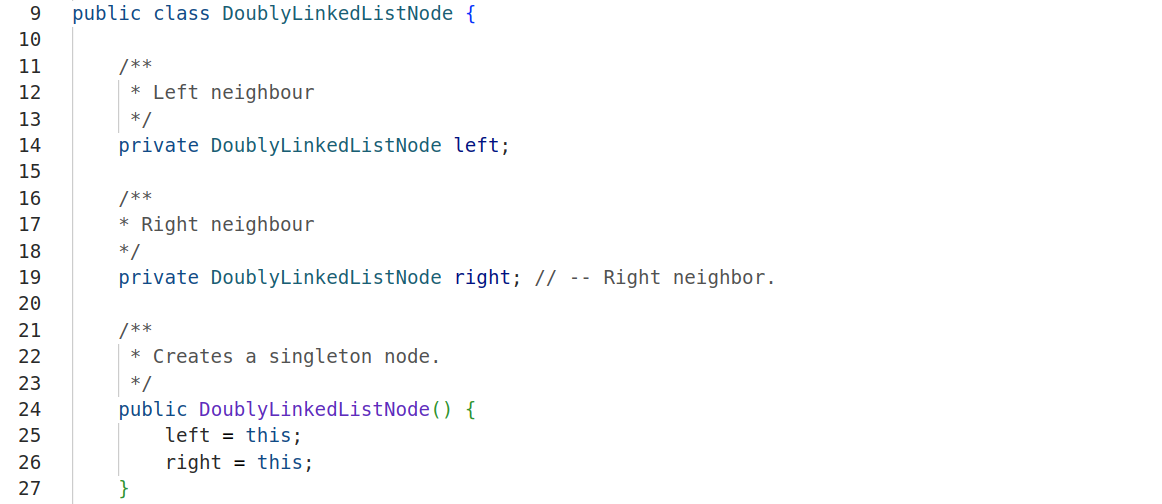
\includegraphics[width=1\textwidth]{doublelinkedlistnode/constructor.png}
\caption{DoubleLinkedListNode}
\label{fig:DoubleLinkedListNode}
\end{figure}


\begin{figure}[ht]
\centering
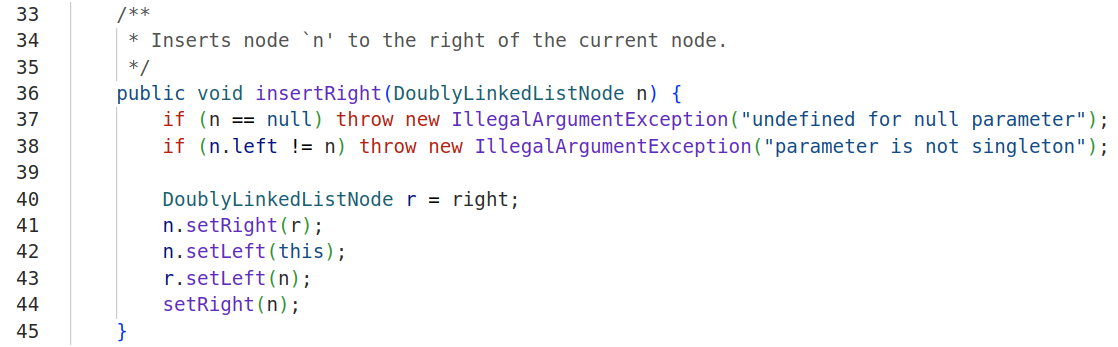
\includegraphics[width=1\textwidth]{doublelinkedlistnode/insertRight.png}
\caption{DoubleLinkedListNode.insertRight}
\label{fig:DoubleLinkedListNodeInsertRight}
\end{figure}

Supongamos ahora que es necesario modificar parte del sistema, y antes de hacerlo sería útil tener aserciones que ayuden a detectar posibles errores que puedan ser insertados durante la actualización con el fin de preservar el comportamiento del sistema.
Para ello se podría considerar automáticamente aserciones de test y de contratos.
En la siguiente imágen se puede ver un caso de test generado por Randoop y un contrato generado por Daikon.

\begin{figure}[ht]
\centering
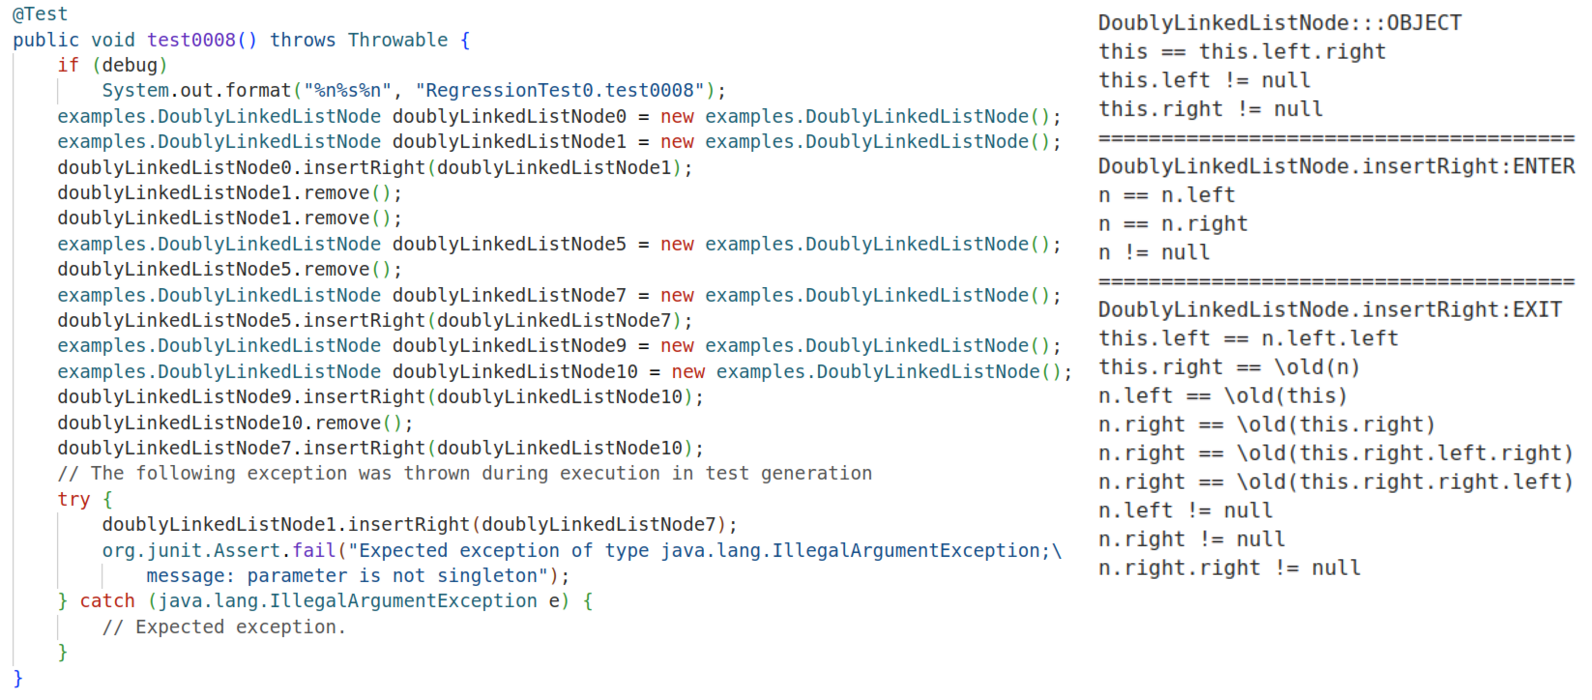
\includegraphics[width=1\textwidth]{doublelinkedlistnode/randoop-daikon-example.png}
\caption{Test y contrato generados automáticamente por Randoop y Daikon respectivamente para el método insertRight}
\label{fig:DoubleLinkedListNodeTests}
\end{figure}

De esta manera, sin demasiado esfuerzo, se han generado automáticamente aserciones que podrían ayudarnos a detectar errores introducidos durante la actualización del sistema. Pero, ¿qué tan efectivos son estas aserciones para detectar errores?. O incluso, ¿cuál tipo de aserción es más eficiente?.

Para dar respuesta a estas preguntas se propone simular escenarios de testing de regresión, introduciendo defectos en el código, técnica conocida como Pruebas de Mutación [], para evaluar la efectividad de las aserciones generadas.